\chapter{动态对冲}
\section{}
\subsection{}

\begin{figure}
    \centering
    \begin{subfigure}{0.45\textwidth}
        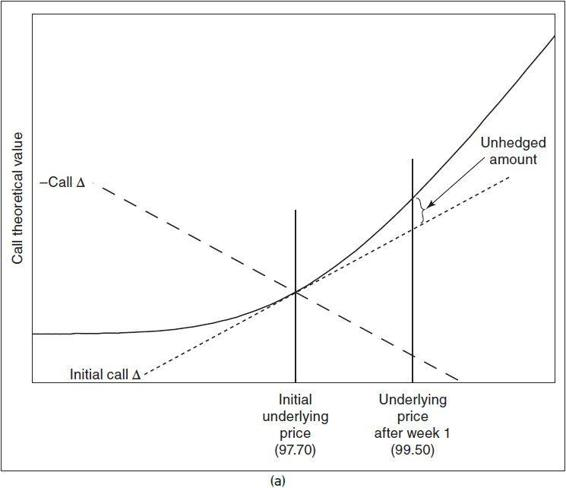
\includegraphics[width=\textwidth]{../img/fig8-3a.png}
        \label{fig8-3a}
    \end{subfigure}
    \hfill
    \begin{subfigure}{0.45\textwidth}
        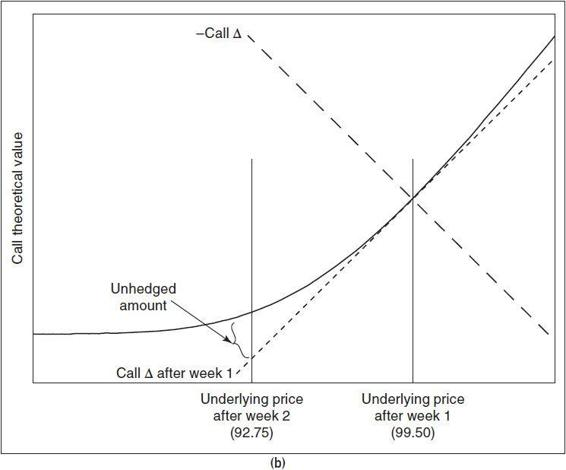
\includegraphics[width=\textwidth]{../img/fig8-3b.png}
        \label{fig8-3b}
    \end{subfigure}
    \caption{我们确定了标的物价格为 97.70 时的期权初始 delta(虚线),然后在标的合约中建立了一个 delta 相反的仓位(虚线)。当标的价格发生很小的变动时,一个仓位的利润可以抵消另一个仓位的损失。由于期权的曲率(其 gamma),当标的价格在任一方向上的变化变大时,这两个仓位之间就会出现不匹配。当标的价格下跌时,期权仓位贬值的速度开始下降;当标的价格上涨时,期权仓位升值的速度开始上升。在 (a) 中,我们可以看到标的价格为 99.50 时的这种不匹配或未对冲金额。当标的价格为 99.50 时,我们通过调整头寸以返回 delta 中性来捕捉这种错配的价值。这如 (b) 所示。我们重新计算了新标的价格下的 delta,并在标的合约中建立了新的对立头寸。当标的价格跌至 92.75 时,错配再次等于未对冲的金额。}
    \label{fig8-3}
\end{figure}

通过重新对冲头寸,我们能够获得一系列利润,这些利润源于期权不断变化的 delta 与标的合约固定 delta 之间的不匹配。当然,在时间流逝的同时,还有利息的考虑。但期权的大部分价值是由重新对冲过程中赚取的金额决定的。理论上,如果我们忽略利息,所有这些小额利润(\autoref{fig8-3} 中未对冲的金额)的总和应该大约等于期权的价值:
$$\text{期权理论价值} = \{\cdot\} + \{\cdot\} + \{\cdot\} + ⋯ + \{\cdot\} + \{\cdot\} + \{\cdot\}$$
